% Options for packages loaded elsewhere
\PassOptionsToPackage{unicode}{hyperref}
\PassOptionsToPackage{hyphens}{url}
%
\documentclass[
]{report}
\usepackage{amsmath,amssymb}
\usepackage{lmodern}
\usepackage{ifxetex,ifluatex}
\ifnum 0\ifxetex 1\fi\ifluatex 1\fi=0 % if pdftex
  \usepackage[T1]{fontenc}
  \usepackage[utf8]{inputenc}
  \usepackage{textcomp} % provide euro and other symbols
\else % if luatex or xetex
  \usepackage{unicode-math}
  \defaultfontfeatures{Scale=MatchLowercase}
  \defaultfontfeatures[\rmfamily]{Ligatures=TeX,Scale=1}
\fi
% Use upquote if available, for straight quotes in verbatim environments
\IfFileExists{upquote.sty}{\usepackage{upquote}}{}
\IfFileExists{microtype.sty}{% use microtype if available
  \usepackage[]{microtype}
  \UseMicrotypeSet[protrusion]{basicmath} % disable protrusion for tt fonts
}{}
\makeatletter
\@ifundefined{KOMAClassName}{% if non-KOMA class
  \IfFileExists{parskip.sty}{%
    \usepackage{parskip}
  }{% else
    \setlength{\parindent}{0pt}
    \setlength{\parskip}{6pt plus 2pt minus 1pt}}
}{% if KOMA class
  \KOMAoptions{parskip=half}}
\makeatother
\usepackage{xcolor}
\IfFileExists{xurl.sty}{\usepackage{xurl}}{} % add URL line breaks if available
\IfFileExists{bookmark.sty}{\usepackage{bookmark}}{\usepackage{hyperref}}
\hypersetup{
  pdftitle={React Notes},
  pdfauthor={Kamal Sacranie},
  hidelinks,
  pdfcreator={LaTeX via pandoc}}
\urlstyle{same} % disable monospaced font for URLs
\usepackage[margin=2cm]{geometry}
\usepackage{color}
\usepackage{fancyvrb}
\newcommand{\VerbBar}{|}
\newcommand{\VERB}{\Verb[commandchars=\\\{\}]}
\DefineVerbatimEnvironment{Highlighting}{Verbatim}{commandchars=\\\{\}}
% Add ',fontsize=\small' for more characters per line
\usepackage{framed}
\definecolor{shadecolor}{RGB}{248,248,248}
\newenvironment{Shaded}{\begin{snugshade}}{\end{snugshade}}
\newcommand{\AlertTok}[1]{\textcolor[rgb]{0.94,0.16,0.16}{#1}}
\newcommand{\AnnotationTok}[1]{\textcolor[rgb]{0.56,0.35,0.01}{\textbf{\textit{#1}}}}
\newcommand{\AttributeTok}[1]{\textcolor[rgb]{0.77,0.63,0.00}{#1}}
\newcommand{\BaseNTok}[1]{\textcolor[rgb]{0.00,0.00,0.81}{#1}}
\newcommand{\BuiltInTok}[1]{#1}
\newcommand{\CharTok}[1]{\textcolor[rgb]{0.31,0.60,0.02}{#1}}
\newcommand{\CommentTok}[1]{\textcolor[rgb]{0.56,0.35,0.01}{\textit{#1}}}
\newcommand{\CommentVarTok}[1]{\textcolor[rgb]{0.56,0.35,0.01}{\textbf{\textit{#1}}}}
\newcommand{\ConstantTok}[1]{\textcolor[rgb]{0.00,0.00,0.00}{#1}}
\newcommand{\ControlFlowTok}[1]{\textcolor[rgb]{0.13,0.29,0.53}{\textbf{#1}}}
\newcommand{\DataTypeTok}[1]{\textcolor[rgb]{0.13,0.29,0.53}{#1}}
\newcommand{\DecValTok}[1]{\textcolor[rgb]{0.00,0.00,0.81}{#1}}
\newcommand{\DocumentationTok}[1]{\textcolor[rgb]{0.56,0.35,0.01}{\textbf{\textit{#1}}}}
\newcommand{\ErrorTok}[1]{\textcolor[rgb]{0.64,0.00,0.00}{\textbf{#1}}}
\newcommand{\ExtensionTok}[1]{#1}
\newcommand{\FloatTok}[1]{\textcolor[rgb]{0.00,0.00,0.81}{#1}}
\newcommand{\FunctionTok}[1]{\textcolor[rgb]{0.00,0.00,0.00}{#1}}
\newcommand{\ImportTok}[1]{#1}
\newcommand{\InformationTok}[1]{\textcolor[rgb]{0.56,0.35,0.01}{\textbf{\textit{#1}}}}
\newcommand{\KeywordTok}[1]{\textcolor[rgb]{0.13,0.29,0.53}{\textbf{#1}}}
\newcommand{\NormalTok}[1]{#1}
\newcommand{\OperatorTok}[1]{\textcolor[rgb]{0.81,0.36,0.00}{\textbf{#1}}}
\newcommand{\OtherTok}[1]{\textcolor[rgb]{0.56,0.35,0.01}{#1}}
\newcommand{\PreprocessorTok}[1]{\textcolor[rgb]{0.56,0.35,0.01}{\textit{#1}}}
\newcommand{\RegionMarkerTok}[1]{#1}
\newcommand{\SpecialCharTok}[1]{\textcolor[rgb]{0.00,0.00,0.00}{#1}}
\newcommand{\SpecialStringTok}[1]{\textcolor[rgb]{0.31,0.60,0.02}{#1}}
\newcommand{\StringTok}[1]{\textcolor[rgb]{0.31,0.60,0.02}{#1}}
\newcommand{\VariableTok}[1]{\textcolor[rgb]{0.00,0.00,0.00}{#1}}
\newcommand{\VerbatimStringTok}[1]{\textcolor[rgb]{0.31,0.60,0.02}{#1}}
\newcommand{\WarningTok}[1]{\textcolor[rgb]{0.56,0.35,0.01}{\textbf{\textit{#1}}}}
\usepackage{longtable,booktabs,array}
\usepackage{calc} % for calculating minipage widths
% Correct order of tables after \paragraph or \subparagraph
\usepackage{etoolbox}
\makeatletter
\patchcmd\longtable{\par}{\if@noskipsec\mbox{}\fi\par}{}{}
\makeatother
% Allow footnotes in longtable head/foot
\IfFileExists{footnotehyper.sty}{\usepackage{footnotehyper}}{\usepackage{footnote}}
\makesavenoteenv{longtable}
\usepackage{graphicx}
\makeatletter
\def\maxwidth{\ifdim\Gin@nat@width>\linewidth\linewidth\else\Gin@nat@width\fi}
\def\maxheight{\ifdim\Gin@nat@height>\textheight\textheight\else\Gin@nat@height\fi}
\makeatother
% Scale images if necessary, so that they will not overflow the page
% margins by default, and it is still possible to overwrite the defaults
% using explicit options in \includegraphics[width, height, ...]{}
\setkeys{Gin}{width=\maxwidth,height=\maxheight,keepaspectratio}
% Set default figure placement to htbp
\makeatletter
\def\fps@figure{htbp}
\makeatother
\setlength{\emergencystretch}{3em} % prevent overfull lines
\providecommand{\tightlist}{%
  \setlength{\itemsep}{0pt}\setlength{\parskip}{0pt}}
\setcounter{secnumdepth}{5}
\usepackage{booktabs}
\usepackage{multicol}
\ifluatex
  \usepackage{selnolig}  % disable illegal ligatures
\fi
\usepackage[]{natbib}
\bibliographystyle{apalike}

\title{React Notes}
\author{Kamal Sacranie}
\date{2021-07-13}

\begin{document}
\maketitle

{
\setcounter{tocdepth}{1}
\tableofcontents
}
\hypertarget{preface}{%
\chapter*{Preface}\label{preface}}
\addcontentsline{toc}{chapter}{Preface}

These are my react notes.

\hypertarget{what-is-react}{%
\section{What is React?}\label{what-is-react}}

React is a library for building UI:

\begin{itemize}
\tightlist
\item
  React runs on the client as a single page application abut can be used to
  build full stack apps by communicating with an API
\item
  React is a frontend framework
\item
  React has a whole bunch of plugins that allow you to do a lote more
\end{itemize}

\hypertarget{why-use-react}{%
\section{Why use react}\label{why-use-react}}

React allows the best way to build your UI using different components which
allows for very dynamic HTML within JavaScript. It does this using JSX (which
is extended JS). React uses what is called the Virtual DOM which allows us to
have a more dymic environment etc.

With react, you'll look at your UI as a bunch of components which you will
write code for.

\hypertarget{creating-a-react-app}{%
\chapter{Creating a React app}\label{creating-a-react-app}}

To create our boilerplate code, we want to use something called `Create React App'.

To install this we want to run \texttt{npx\ create-react-app\ \textless{}app-name\textgreater{}}. This uses the node package manager so \textbf{Node must be installed}. This sets up our frontend.

In these created files we have \texttt{package.json} which tells us exactly what dependencies/addons are installed in React and we \textbf{change this when we add an extension} (this wil ususally be in the docs of the extension)

\hypertarget{what-we-get-in-our-boilerplate}{%
\subsection{What we get in our boilerplate}\label{what-we-get-in-our-boilerplate}}

We get an \texttt{index.html} which basically just has a body tag with \texttt{\textless{}div\ id="root"\textgreater{}\textless{}/div\textgreater{}} which is basically the crux of how our React app gets rendered.

In the \texttt{src} folder, inside the \texttt{index.js} which is our front-most part of our React app, we grab the \texttt{root} elemtent from our \texttt{index.html} and render our \texttt{\textless{}App\ /\textgreater{}}. This \texttt{\textless{}App\ /\textgreater{}} tag comes from importing our root app from \texttt{App.js} which houses all of our components. Basically:

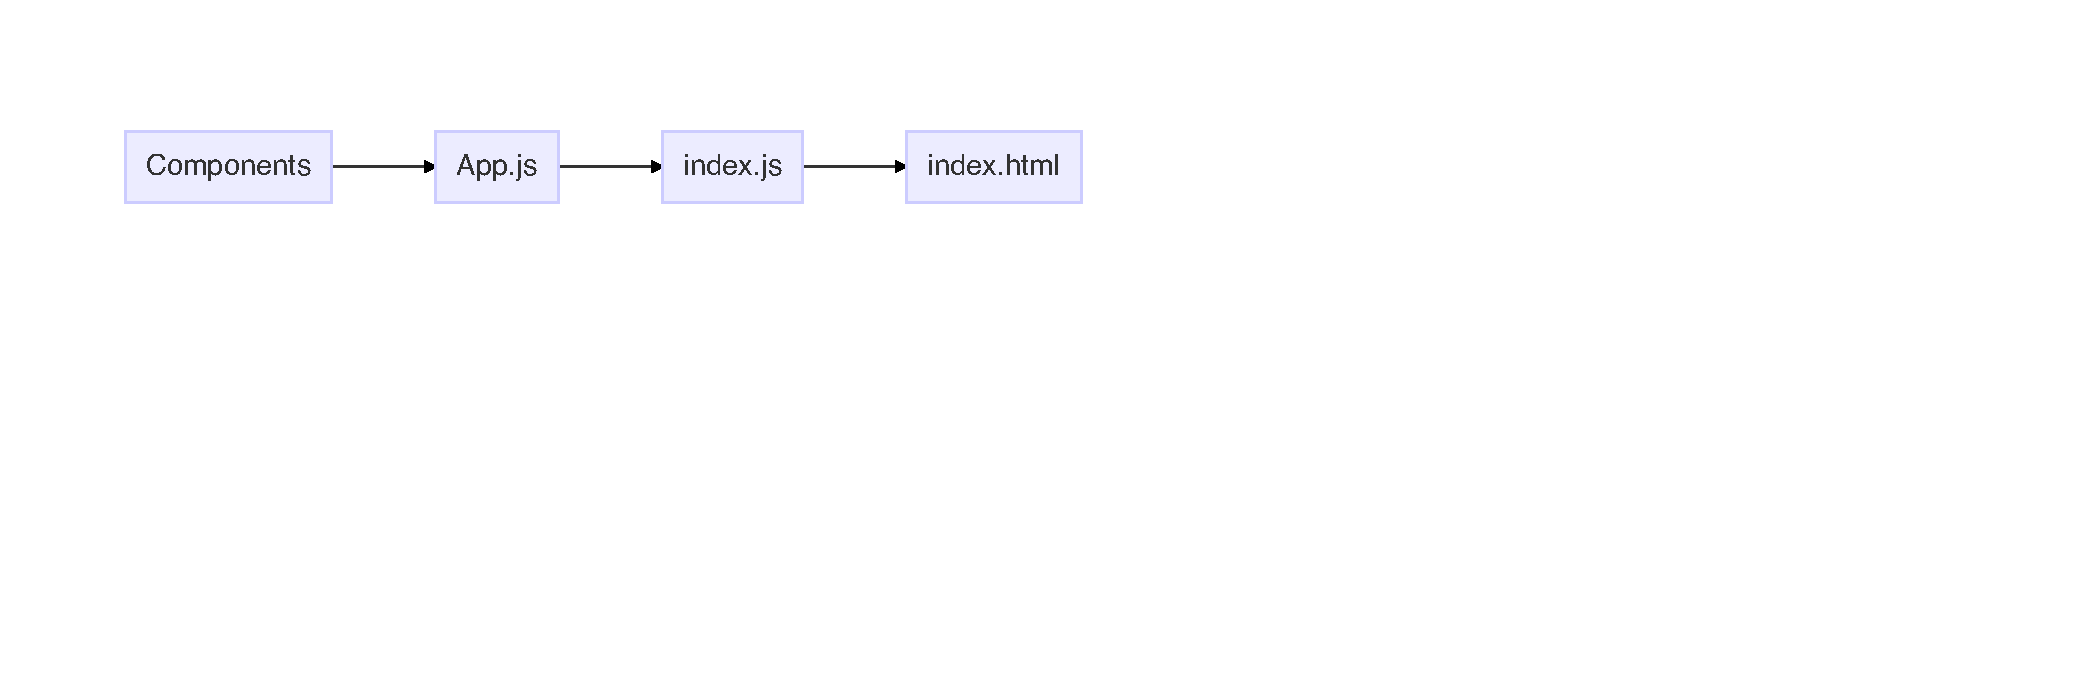
\includegraphics{react-notes_files/figure-latex/unnamed-chunk-1-1.pdf}

\hypertarget{starting-up-our-dev-server}{%
\subsection{Starting up our dev server}\label{starting-up-our-dev-server}}

You must change directory into your React app folder and then we can run \texttt{npm\ start} which will start our server on \textbf{localhost:3000}.

\hypertarget{components}{%
\section{Components}\label{components}}

In react, you can create components with funcitons and classes. The more common
way these days is to \textbf{use functions}. Class components extend other classes.

Your basic functional component looks as follows:

\begin{Shaded}
\begin{Highlighting}[]
\KeywordTok{let}\NormalTok{ myVar}\OperatorTok{;}

\ImportTok{export} \KeywordTok{const}\NormalTok{ Header }\OperatorTok{=}\NormalTok{ () }\KeywordTok{=\textgreater{}}\NormalTok{ \{}
    \ControlFlowTok{return}\NormalTok{ (}
        \OperatorTok{\textless{}}\NormalTok{some HTML}\OperatorTok{\textgreater{}}
\NormalTok{            \{myVar\}}
\NormalTok{            \{}\DecValTok{1} \OperatorTok{+} \DecValTok{2}\NormalTok{\} }\CommentTok{// This will render as 3}
        \OperatorTok{\textless{}/}\NormalTok{some HTML}\OperatorTok{\textgreater{}}
\NormalTok{    )}
\NormalTok{\}}
\end{Highlighting}
\end{Shaded}

\begin{itemize}
\tightlist
\item
  Because we use the component in other \texttt{.js} files, we use the \texttt{export} keyword to denote that we are exporting the component for use elsewhere.
\item
  We are also using arrow funciton here
\item
  Note that the return is returning HTML. This isn't really HTML but rather JSX (JavaScript Syntax Extension) which allows us to use HTML and any JS expression to make our pseudo-HTML dynamic.
\item
  We also see that we can have JS varaibels inside curly braces
\item
  You must also only return one single top level element
\end{itemize}

You can also pass in `props' to your components which allows you to pass data into your components which can be used.

Components have what is known as `state' which is an object that determines how a component renders and behaves. This could be a value like `opne' or `close'. Sometimes you want App level state which referes to state that is available to the entire UI and not just a single component. This is done through Redux.

\begin{quote}
In React and JSX, we \textbf{have clashes} of HTML tag attributes like \texttt{class} and \texttt{for}, to get around this we use \texttt{className} and \texttt{htmlFor} respectively.
\end{quote}

\hypertarget{creating-components}{%
\subsection{Creating components}\label{creating-components}}

We create our components inside our \texttt{src} file inside a \texttt{components} file as \texttt{.js} files.

You can use VSCode snippets addon to create the boilerplate for a component which will look as follows:

\begin{Shaded}
\begin{Highlighting}[]
\KeywordTok{const}\NormalTok{ MyComponent }\OperatorTok{=}\NormalTok{ () }\KeywordTok{=\textgreater{}}\NormalTok{ \{}
    \ControlFlowTok{return}\NormalTok{ (}
        \OperatorTok{\textless{}}\NormalTok{html}\OperatorTok{\textgreater{}}
        \OperatorTok{\textless{}/}\NormalTok{html}\OperatorTok{\textgreater{}} 
\NormalTok{    )}
\NormalTok{\}}

\ImportTok{export} \ImportTok{default}\NormalTok{ MyComponent}
\end{Highlighting}
\end{Shaded}

\begin{quote}
Note that we name our components in proper case.
\end{quote}

We must then import it into our \texttt{App.js}:

\begin{Shaded}
\begin{Highlighting}[]
\ImportTok{import}\NormalTok{ MyComponent }\ImportTok{from} \StringTok{\textquotesingle{}./componennets/MyComponent\textquotesingle{}}

\KeywordTok{function} \FunctionTok{App}\NormalTok{() \{}
    \ControlFlowTok{return}\NormalTok{ (}
        \OperatorTok{\textless{}}\NormalTok{div}\OperatorTok{\textgreater{}}
            \OperatorTok{\textless{}}\NormalTok{MyComponent }\OperatorTok{/\textgreater{}} \CommentTok{// calling our component here}
        \OperatorTok{\textless{}/}\NormalTok{div}\OperatorTok{\textgreater{}}
\NormalTok{    )}
\NormalTok{\}}
\end{Highlighting}
\end{Shaded}

\begin{itemize}
\tightlist
\item
  Notice here that when we import we use quotes for te path name
\item
  We \textbf{call our component with \texttt{\textless{}ComponentName\ /\textgreater{}}}
\end{itemize}

\hypertarget{props}{%
\section{Props}\label{props}}

Props are basically parameters for your functional componenets which are \textbf{passed in through the tag}. We can access it in our component as an object.

\begin{Shaded}
\begin{Highlighting}[]
\KeywordTok{const}\NormalTok{ MyComponent }\OperatorTok{=}\NormalTok{ (props) }\KeywordTok{=\textgreater{}}\NormalTok{ \{}
    \ControlFlowTok{return}\NormalTok{ (}
        \OperatorTok{\textless{}}\NormalTok{html}\OperatorTok{\textgreater{}}
            \OperatorTok{\textless{}}\NormalTok{h1}\OperatorTok{\textgreater{}\textless{}/}\NormalTok{h1}\OperatorTok{\textgreater{}}
        \OperatorTok{\textless{}/}\NormalTok{html}\OperatorTok{\textgreater{}} 
\NormalTok{    )}
\NormalTok{\}}

\CommentTok{// ====== In the file where we call the component ====}

\OperatorTok{\textless{}}\NormalTok{MyComponent title}\OperatorTok{=}\StringTok{\textquotesingle{}Hello\textquotesingle{}}\OperatorTok{\textgreater{}}
\end{Highlighting}
\end{Shaded}

\begin{itemize}
\tightlist
\item
  As you can see, you do not need to expliclity define \texttt{title} but can pass it in and access it from a dictionary.
\end{itemize}

\hypertarget{default-props}{%
\subsection{Default props}\label{default-props}}

We can have default props for our components by doing the following:

\begin{Shaded}
\begin{Highlighting}[]
\KeywordTok{const}\NormalTok{ MyComponent }\OperatorTok{=}\NormalTok{ (\{ title \}) }\KeywordTok{=\textgreater{}}\NormalTok{ \{}
    \ControlFlowTok{return}\NormalTok{ (}
        \OperatorTok{\textless{}}\NormalTok{html}\OperatorTok{\textgreater{}}
            \OperatorTok{\textless{}}\NormalTok{h1}\OperatorTok{\textgreater{}}\NormalTok{title}\OperatorTok{\textless{}/}\NormalTok{h1}\OperatorTok{\textgreater{}}
        \OperatorTok{\textless{}/}\NormalTok{html}\OperatorTok{\textgreater{}} 
\NormalTok{    )}
\NormalTok{\}}

\NormalTok{Header}\OperatorTok{.}\AttributeTok{defaultProps} \OperatorTok{=}\NormalTok{ \{}
    \DataTypeTok{title}\OperatorTok{:} \StringTok{\textquotesingle{}My Title\textquotesingle{}}
\NormalTok{\}}
\end{Highlighting}
\end{Shaded}

\begin{itemize}
\tightlist
\item
  Note that here we have descructured the object by using the \{\} which allows us to just directly access title.
\end{itemize}

We can also \texttt{import\ PropTypes\ form\ \textquotesingle{}prop-types\textquotesingle{}} to typeset your props using KVPs in the object \texttt{MyComponent.propTypes\ =\ \{title:\ PropType.string\}}

\hypertarget{componenets-in-components}{%
\subsection{Componenets in components}\label{componenets-in-components}}

It is simple to have components within components, all you have to do is
perform the relative import in your current component and the component will be
in the same directory so its just \texttt{\textquotesingle{}./Component}.

\hypertarget{styles}{%
\chapter{Styles}\label{styles}}

\hypertarget{in-line-styles}{%
\section{In-line styles}\label{in-line-styles}}

If we are going to add styles inline in one of our React componenets, we can use the fact that JSX allows for HTML/CSS. This is donw within a tag using double curly braces:

\begin{Shaded}
\begin{Highlighting}[]
\KeywordTok{const}\NormalTok{ Component }\OperatorTok{=}\NormalTok{ () }\KeywordTok{=\textgreater{}}\NormalTok{ \{}
    \ControlFlowTok{return}\NormalTok{ (}
        \OperatorTok{\textless{}}\NormalTok{h1 style}\OperatorTok{=}\NormalTok{\{\{ }\DataTypeTok{backgroundColor}\OperatorTok{:} \StringTok{\textquotesingle{}black\textquotesingle{}}\OperatorTok{,} \DataTypeTok{color}\OperatorTok{:} \StringTok{\textquotesingle{}red\textquotesingle{}}\NormalTok{ \}\}}\OperatorTok{\textgreater{}}
        \OperatorTok{\textless{}/}\NormalTok{h1}\OperatorTok{\textgreater{}}
\NormalTok{    )}
\end{Highlighting}
\end{Shaded}

\begin{itemize}
\tightlist
\item
  Note here that we use double curly braces
\item
  We also have CSS elements in camelCase
\item
  Style elements are also seperated by \texttt{,} not \texttt{;}
\end{itemize}

\hypertarget{via-a-variable-in-the-same-js-file}{%
\section{Via a variable in the same JS file}\label{via-a-variable-in-the-same-js-file}}

This is pretty self explanitary. We can just create an object somewhere else in our JS document and add the style inline using the constant keyword that we created.

\hypertarget{using-a-css-file}{%
\section{Using a CSS file}\label{using-a-css-file}}

Using a CSS file is pretty simple, you just relate the link in your \texttt{index.html} file.

\hypertarget{create-state-without-redux}{%
\chapter{Create state without Redux}\label{create-state-without-redux}}

To create state without Redux, we can create a component containing the data we
want to use and import the \texttt{useState} function from React:

\begin{Shaded}
\begin{Highlighting}[]
\ImportTok{import}\NormalTok{ \{ useState \} }\ImportTok{from} \StringTok{\textquotesingle{}react\textquotesingle{}}

\KeywordTok{const}\NormalTok{ Data }\OperatorTok{=}\NormalTok{ () }\KeywordTok{=\textgreater{}}\NormalTok{ \{}
    \KeywordTok{const}\NormalTok{ [data}\OperatorTok{,}\NormalTok{ setData] }\OperatorTok{=} \FunctionTok{useState}\NormalTok{(}\OperatorTok{\textless{}}\NormalTok{myObjectOfData}\OperatorTok{\textgreater{}}\NormalTok{)}
    
    \ControlFlowTok{return}\NormalTok{ (}
        \OperatorTok{\textless{}\textgreater{}}
\NormalTok{            \{data}\OperatorTok{.}\FunctionTok{map}\NormalTok{((task) }\KeywordTok{=\textgreater{}}\NormalTok{ (}
                \OperatorTok{\textless{}}\NormalTok{li key}\OperatorTok{=}\NormalTok{\{data}\OperatorTok{.}\AttributeTok{id}\NormalTok{\}}\OperatorTok{\textgreater{}}\NormalTok{\{data}\OperatorTok{.}\AttributeTok{text}\NormalTok{\}}\OperatorTok{\textless{}/}\NormalTok{li}\OperatorTok{\textgreater{}}
\NormalTok{            ))\}}
        \OperatorTok{\textless{}/\textgreater{}}
\NormalTok{    )}
\NormalTok{\}}
\end{Highlighting}
\end{Shaded}

\begin{itemize}
\tightlist
\item
  Here we are importing \texttt{useState} and then using it to properly assign data to a variable
\item
  We also use the map function to basically perform a for each loop on our data and then pass in the function we want to perform with each entry of data
\item
  We also pass in a \texttt{key} attribute which is required for React
\end{itemize}

We don't typically want our data in to be in one component however, so we typically use Redux to create a state which is avaialbe to all of our components. For small projects which we don't want to use Redux for, we can put the data in our \texttt{App.js} file to emulate a global state and pass it through as props to our components.

To update our immutable state we use \texttt{setData} which we defined in \ref{exm:setting-state} which is a funciton that we can use with \texttt{filter()} to change our state. Basically if we want to do something like this we can Google it on the spot.

\begin{quote}
If you set the state within your functional component using \texttt{useState()} it is what is known as component level state.
\end{quote}

\hypertarget{the-usestate-function}{%
\section{\texorpdfstring{The \texttt{useState} function}{The useState function}}\label{the-usestate-function}}

What the \texttt{useState} function actually does is:

\begin{enumerate}
\def\labelenumi{\arabic{enumi}.}
\tightlist
\item
  It takes in our default state, and returns an array with 2 entries.
\item
  The first element is \textbf{our state} which we passed into \texttt{useState} and the
  second element is \textbf{a function which allows us to update our state later}
\end{enumerate}

An example of how we would update our sate would be if we did the following in
\texttt{App.js}:

\begin{Shaded}
\begin{Highlighting}[]
\ImportTok{import}\NormalTok{ \{ useState \} }\ImportTok{from} \StringTok{\textquotesingle{}react\textquotesingle{}}

\KeywordTok{function} \FunctionTok{App}\NormalTok{() \{}
    \KeywordTok{const}\NormalTok{ [count}\OperatorTok{,}\NormalTok{ setCount] }\OperatorTok{=} \FunctionTok{useStata}\NormalTok{(}\DecValTok{4}\NormalTok{)}

    \KeywordTok{const}\NormalTok{ decrementCount }\OperatorTok{=}\NormalTok{ () }\KeywordTok{=\textgreater{}}\NormalTok{ \{}
        \FunctionTok{setCount}\NormalTok{(previousCount }\KeywordTok{=\textgreater{}}\NormalTok{ prevCount }\OperatorTok{{-}} \DecValTok{1}\NormalTok{)}
\NormalTok{    \}}

    \ControlFlowTok{return}\NormalTok{ (}
        \OperatorTok{\textless{}\textgreater{}}
            \OperatorTok{\textless{}}\NormalTok{button onClick}\OperatorTok{=}\NormalTok{\{decrementCount\}}\OperatorTok{\textgreater{}{-}\textless{}/}\NormalTok{button}\OperatorTok{\textgreater{}}
            \OperatorTok{\textless{}}\NormalTok{span}\OperatorTok{\textgreater{}}\NormalTok{\{count\}}\OperatorTok{\textless{}/}\NormalTok{span}\OperatorTok{\textgreater{}}
            \OperatorTok{\textless{}}\NormalTok{button}\OperatorTok{\textgreater{}+\textless{}/}\NormalTok{button}\OperatorTok{\textgreater{}}
        \OperatorTok{\textless{}/\textgreater{}}
\NormalTok{    )}
\NormalTok{\}}
\end{Highlighting}
\end{Shaded}

\begin{itemize}
\tightlist
\item
  Here we \textbf{desructure} our array response from \texttt{useState} into \texttt{count} and
  \texttt{setCount}.
\item
  We then create a function which runs on the click of the button which
  decreases our count
\item
  When the page loads, we load in our default state which is \texttt{4}
\item
  Every time we call the \texttt{decrementCount} our component rerenders our component
\item
  Any time you are modifying your state incrementally you must pass in a
  function to our \texttt{setCount} function which is what the react docs say
\end{itemize}

Use state can also take a function input which atually \textbf{only runs once} which
is good for the performance of our webpage. For this to happen you have to pass
the function directly in and not reference the function.

\hypertarget{the-useeffect-function}{%
\section{\texorpdfstring{The \texttt{useEffect} function}{The useEffect function}}\label{the-useeffect-function}}

Use effect basically handles side effects and it takes a function as an
argument. \texttt{useEffect} is commonly used with asyn await to get a response from a
backend like for example when using Django we would do the fillowing:

\begin{Shaded}
\begin{Highlighting}[]
\KeywordTok{const}\NormalTok{ App }\OperatorTok{=}\NormalTok{ () }\KeywordTok{=\textgreater{}}\NormalTok{ \{}

\CommentTok{// code}

    \FunctionTok{useEffect}\NormalTok{(() }\KeywordTok{=\textgreater{}}\NormalTok{ \{}
        \KeywordTok{const}\NormalTok{ fetchData }\OperatorTok{=} \KeywordTok{async}\NormalTok{ () }\KeywordTok{=\textgreater{}}\NormalTok{ \{}
            \KeywordTok{const}\NormalTok{ data }\OperatorTok{=} \ControlFlowTok{await}\NormalTok{ axios}\OperatorTok{.}\FunctionTok{get}\NormalTok{(}\StringTok{\textquotesingle{}path/to/endpoint\textquotesingle{}}\NormalTok{)}
\NormalTok{        \}}
        \FunctionTok{fetchData}\NormalTok{()}
\NormalTok{    \}}\OperatorTok{,}\NormalTok{ [])}
\NormalTok{\}}
\end{Highlighting}
\end{Shaded}

\begin{itemize}
\tightlist
\item
  Basically we've fetched the data from our backend to use in our React
  component. We have then called the \texttt{fetchData} function to got our data
\item
  We then passin an empty array as a second argument which usually takes values
  which we want useEffect to run when the value changes
\end{itemize}

\hypertarget{static-assets}{%
\chapter{Static assets}\label{static-assets}}

If we are ready to deploy, we can run \texttt{npm\ run\ build} which creates a build in
a folder called build. Basically all our react gets converted to vanilla JS
which we can deploy. So basically we would deploy the files in the build
folder.

You can go about deploying your files in many different ways. Anything that
hosts JS, HTML, and CSS static files can host regular react apps. If you have a
database, it becomes a bit harder to host because you need a server to run your
backend.

\hypertarget{routing-in-react}{%
\chapter{Routing in React}\label{routing-in-react}}

Natively we cannot rout with react and I'm sure there is some way to use Django
for routing but it's easier to just use react router dom. We just need to \texttt{npm\ install\ react-router-dom} which will automatically show up in our \texttt{package.json}which enables us to route.

When we want to create a route we need to \texttt{import\ \{\ BrowserRouter\ as\ Router,\ Route\}\ from\ \textquotesingle{}react-router-dom}. Then we will wrap our whole return statement in
\texttt{App.js} in the \texttt{\textless{}Router\textgreater{}} tag which allows us to then use \texttt{Route}:

\begin{Shaded}
\begin{Highlighting}[]
\NormalTok{cont App }\OperatorTok{=}\NormalTok{ () }\KeywordTok{=\textgreater{}}\NormalTok{ \{}
    \ControlFlowTok{return}\NormalTok{ (}
        \OperatorTok{\textless{}}\NormalTok{Router}\OperatorTok{\textgreater{}}
            \CommentTok{// HTML}
            \OperatorTok{\textless{}}\NormalTok{Route }
\NormalTok{                path}\OperatorTok{=}\StringTok{\textquotesingle{}/\textquotesingle{}} 
\NormalTok{                exact }
\NormalTok{                render}\OperatorTok{=}\NormalTok{\{(props) }\KeywordTok{=\textgreater{}}\NormalTok{ (}\CommentTok{// what you want to render)\}}
            \OperatorTok{/\textgreater{}}
            \OperatorTok{\textless{}}\NormalTok{Route path}\OperatorTok{=}\StringTok{\textquotesingle{}/about\textquotesingle{}}\NormalTok{ components}\OperatorTok{=}\NormalTok{\{About\} }\OperatorTok{/\textgreater{}}
        \OperatorTok{\textless{}/}\NormalTok{Router}\OperatorTok{\textgreater{}}
\NormalTok{    )}
\NormalTok{\}}
\end{Highlighting}
\end{Shaded}

This basically allows us to selectively render stuff depending on the path so
in essence your webapp is a single page application. This would render
something when we match the \textbf{exact} route of \texttt{/} and then when the route is
\texttt{/about} we would get the about component rendered.

\hypertarget{react-links}{%
\section{React links}\label{react-links}}

This allows us to not reload the page when routing with React. We do this
directly in the component concerned like if we had an about component which
directed us to the home page, we would:

\begin{Shaded}
\begin{Highlighting}[]
\ImportTok{import}\NormalTok{ \{ Link \} }\ImportTok{from} \StringTok{\textquotesingle{}react{-}router{-}dom\textquotesingle{}}

\KeywordTok{const}\NormalTok{ About }\OperatorTok{=}\NormalTok{ () }\KeywordTok{=\textgreater{}}\NormalTok{ \{}
    \ControlFlowTok{return}\NormalTok{ (}
        \OperatorTok{\textless{}\textgreater{}}
            \OperatorTok{\textless{}}\NormalTok{Link to}\OperatorTok{=}\StringTok{\textquotesingle{}/\textquotesingle{}}\OperatorTok{\textgreater{}}\NormalTok{Home}\OperatorTok{\textless{}/}\NormalTok{Link}\OperatorTok{\textgreater{}}
        \OperatorTok{\textless{}/\textgreater{}}
\NormalTok{    )}
\NormalTok{\}}
\end{Highlighting}
\end{Shaded}

\begin{quote}
This would just take us home and not force us to reload the page like we
would with an anchor tag
\end{quote}

\hypertarget{uselocation}{%
\section{\texorpdfstring{\texttt{useLocation}}{useLocation}}\label{uselocation}}

This allows us to use the current URL to selectively render elements depending
on our route. We would \texttt{import\ \{\ useLocation\ \}\ from\ \textquotesingle{}react-router-dom\textquotesingle{}} and
then define a variable which just runs the function which gives us access to
the path name and we can use a conditional to show something depending on the
path.

  \bibliography{../sources/book.bib}

\end{document}
